\section{MisUse Cases}

Was sind Misuse Cases blablabla


\subsection{Misuse Case Diagramme}

allgemein

seamonster

\begin{figure}
\caption{Misuse Case Diagramm für ein Einbruchsszenario. Dem Angreifer werden verschiedene Sicherheitsmaßnahmen entgegengestellt, die einen Einbruch verhindern oder erschweren können}
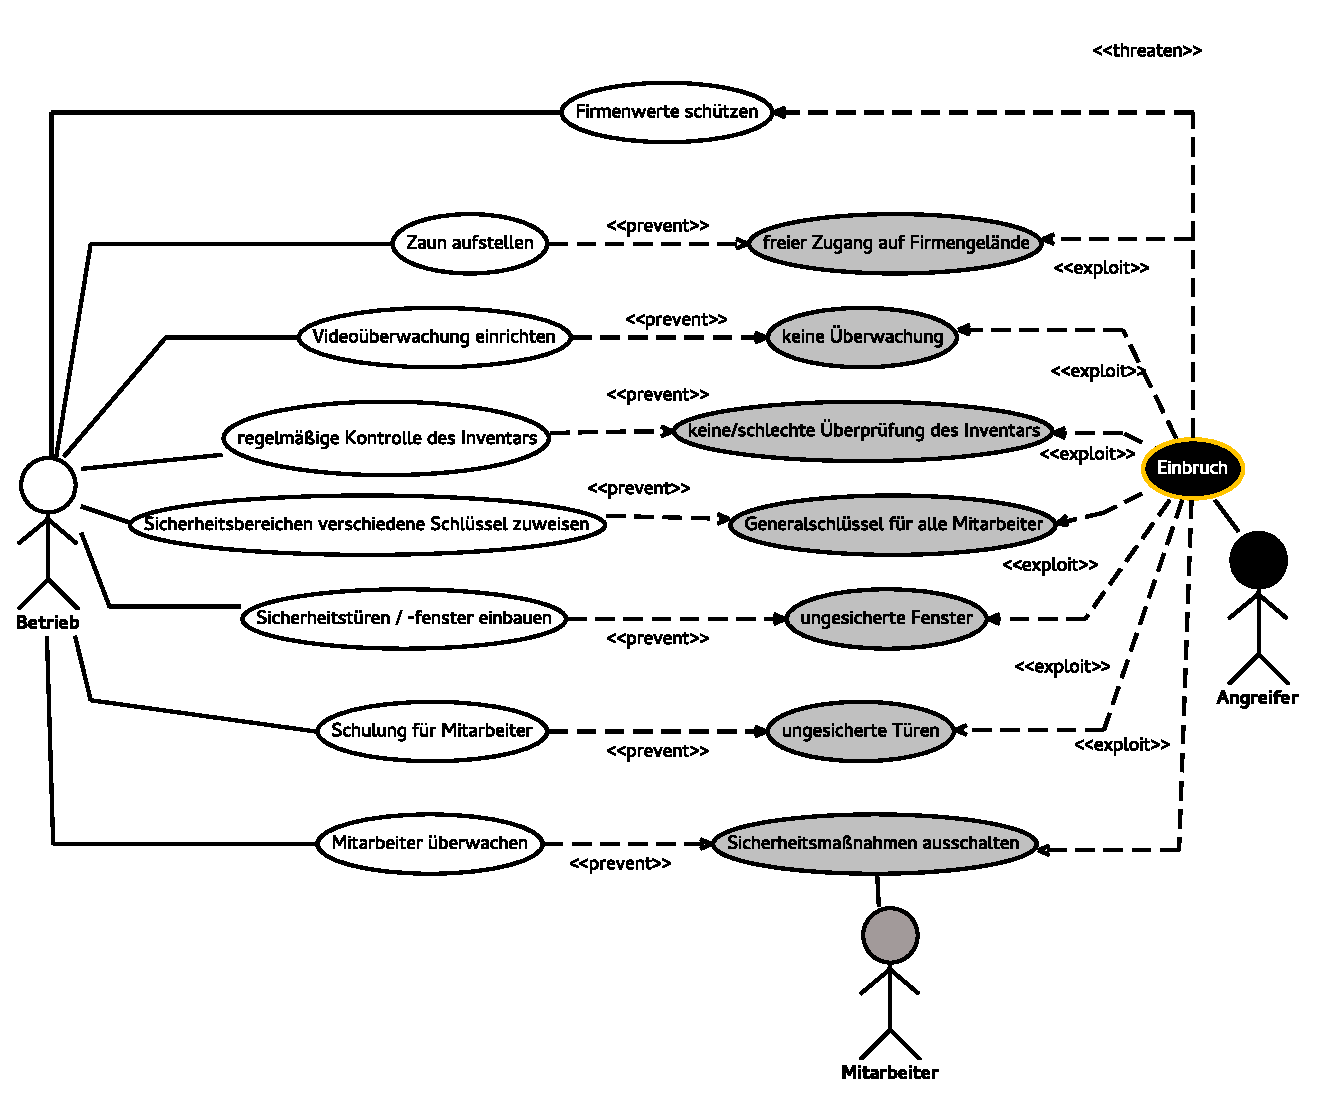
\includegraphics[scale=0.8,angle=90]{images/MisUseCaseEinbruch.pdf} 
\end{figure}

\begin{figure}
\caption{Misuse Case Diagramm für den Missbrauch von Außendienstmitarbeiterhardware. Sicherheitsrichtlinien für Geräte (z.B. Verschlüsselung) können Angriffe erschweren oder verhindern.}
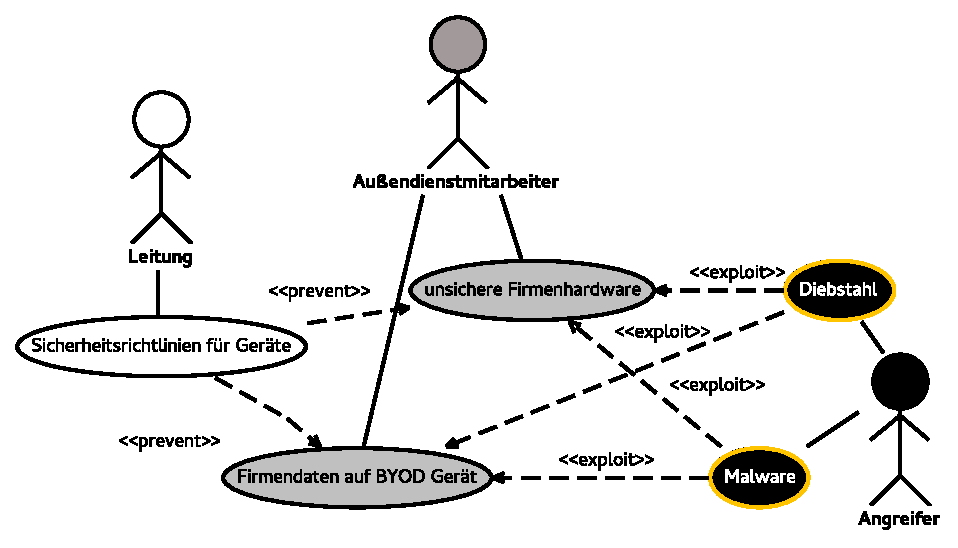
\includegraphics[scale=0.8]{images/Hardware.pdf} 
\end{figure}


\begin{figure}
\caption{Misuse Case Diagramm }
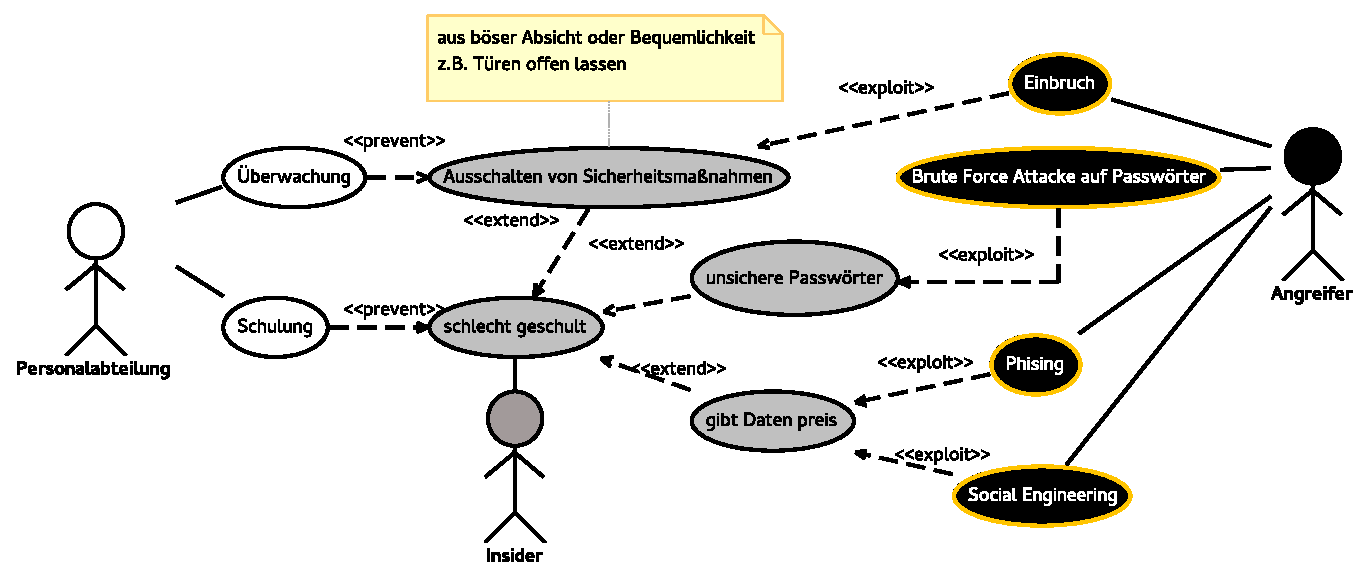
\includegraphics[scale=0.8,angle=90]{images/Schulung.pdf} 
\end{figure}

\begin{figure}
\caption{Misuse Case Diagramm }
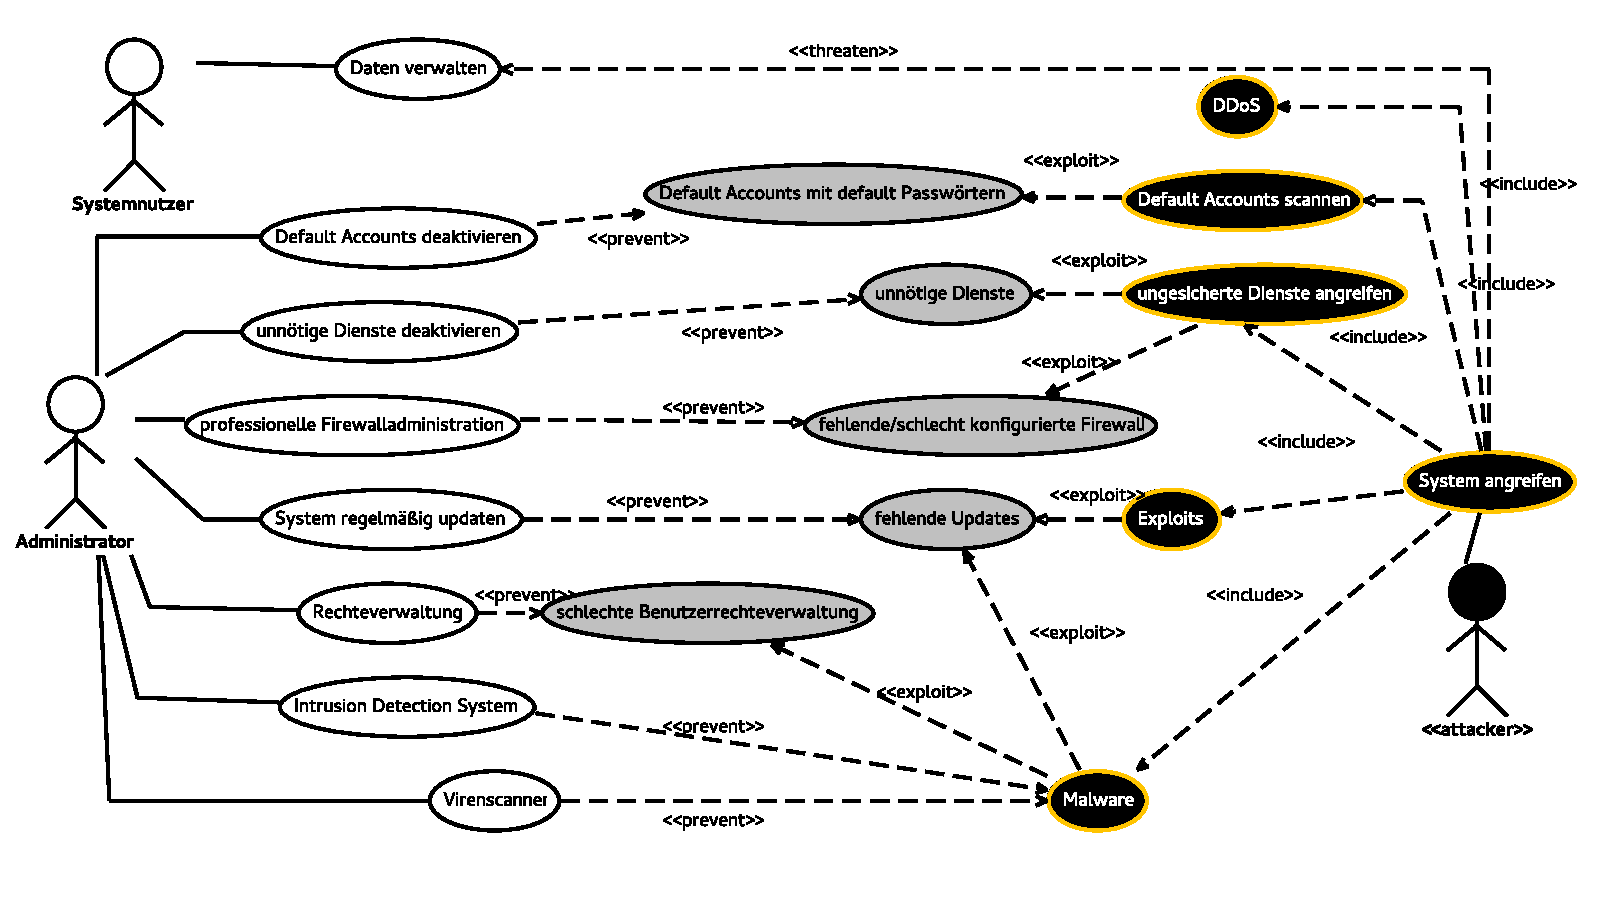
\includegraphics[scale=0.8,angle=90]{images/Server.pdf} 
\end{figure}






\subsection{Vergleich FB I und FB II}

fast gleich